\documentclass{article}
\usepackage{amsmath}
\usepackage{amssymb}
\usepackage[a4paper, top=25mm, bottom=25mm, left=25mm, right=25mm]{geometry}
\usepackage{pgfplots}
\pgfplotsset{compat=1.18}
\usepackage{mathtools}
\usepgfplotslibrary{polar}
\usepgfplotslibrary{fillbetween}

\begin{document}
\pagestyle{empty}
\large

\begin{center}
2022-2023 Spring \\MAT124 Final\\(12/06/2023)
\end{center}

\noindent 1. Maximize the function $f(x,y)=xy^2z$ on the sphere $x^2+y^2+z^2 = 4$.

\hfill

\noindent 2. Sketch the region corresponding to the double integral

\begin{equation*}\int_0^1\int_{x^{1/4}}^1\,\mathrm{e}^{y^5}dy\,dx\end{equation*}

\hfill

\noindent and evaluate it.

\hfill

\noindent 3. Sketch the region $R$ inside the cardioid $r=1+\cos\theta$ and outside the limaçon $r=2-\cos\theta$, and set up the polar double integral corresponding to the area of the region $R$.

\hfill

\noindent 4. Using a double integral, find the volume of the solid bounded above by the elliptic paraboloid $z=4-x^2-y^2$ and below by the circular region $x^2+y^2\leq2$ in the $xy$-plane where $x\geq0$ and $y\geq0$.

\hfill

\noindent 5. Let us consider the frustum of the cone $z=\sqrt{x^2+y^2}$ between the planes $z=1$ and $z=2$.

\hfill

\noindent (i) Sketch the graph of the frustum.

\hfill

\noindent (ii) Find the surface area of the frustum.

\hfill

\noindent 6. Let $S$ be the region in the cylinder $x^2+y^2 = 1$ bounded above by the plane $z=4$ and below by the sphere $x^2+y^2+z^2=1$.

\hfill

\noindent (i) Using the spherical coordinates, set up (but do not evaluate!) an integral for the volume of the solid $S$.

\hfill

\noindent (ii) Using the cylindrical coordinates, find the volume of the solid $S$.

\newpage

\begin{center}
2022-2023 Spring Final (12/06/2023) Solutions\\
(Last update: 05/08/2025 00:53)
\end{center}

\noindent 1. Let $g(x,y,z)=x^2+y^2+z^2-4$ and then solve the system of equations below using the method of Lagrange multipliers.

\[
\left.
\begin{array}{ll}
\displaystyle\nabla f =\lambda \nabla g \\
\displaystyle g(x,y,z) = 0
\end{array}
\right\}\quad
\begin{array}{ll}
\nabla f = \left\langle y^2z,2xyz,xy^2\right\rangle = \lambda\left\langle2x,2y,2z\right\rangle = \lambda\nabla g \\[0.2cm] x^2+y^2+z^2-4=0
\end{array}
\]

\[
\left.
\begin{array}{ll}
\displaystyle y^2z =\lambda \cdot2x & (1)\\[0.2cm]
\displaystyle 2xyz =\lambda \cdot2y & (2)\\[0.2cm]
\displaystyle xy^2 =\lambda \cdot2z & (3)\\[0.2cm]
\end{array}
\right\}\quad
\begin{array}{ll}
\displaystyle(1)\,\&\,(3)\rightarrow\frac{z}{x}=\frac{x}{z}\rightarrow x^2=z^2\rightarrow x=\pm z&(4)\\[0.4cm]
\displaystyle(1)\,\&\,(2)\rightarrow\frac{y}{2x}=\frac{x}{y}\rightarrow y^2=2x^2\rightarrow y=\pm\sqrt{2}x&(5)\\[0.4cm]\displaystyle(4)\,\&\,(5)\rightarrow y=\pm \sqrt 2z
\end{array}
\]

\hfill

\noindent Now, use the constraint to find the coordinates. Write $y$ and $z$ in terms of $x$.

\[x^2+y^2+z^2-4=0\implies x^2+\left(\sqrt2x\right)^2+x^2-4=0\implies4x^2=4\implies x=\pm1\]
\[\therefore y=\pm\sqrt2,\quad z=\pm1\]

\hfill

\noindent Evaluate $f$ at either of these points: $(1,\sqrt2,1)$, $(-1,\sqrt2,-1)$, $(-1,-\sqrt2,-1)$.

\[f_{\text{max}}=f(1,\sqrt2,1)=1\cdot\left(\sqrt2\right)^2\cdot1=\boxed{2}\]

\hfill

\noindent 2.

\begin{center}
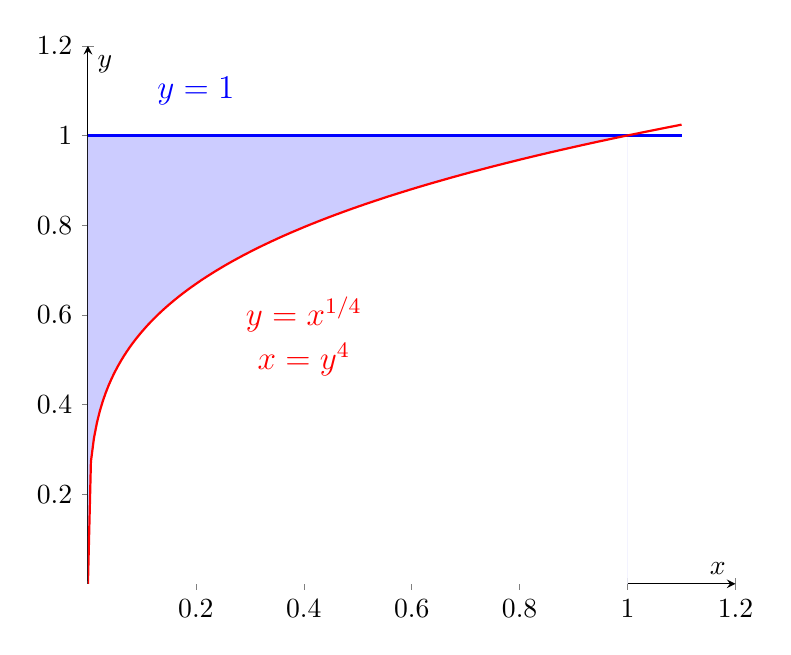
\begin{tikzpicture}
  \begin{axis}[
      axis lines=center,
      xlabel={$x$},
      ylabel={$y$},
      xmin=0, xmax=1.2,
      ymin=0, ymax=1.2,
      samples=200,
      clip=true,
      scale=1.2,
    ]
    
    \addplot [
        fill=blue!20,
        domain=0:1,
        draw=none,
    ] {1} \closedcycle;
    
    \addplot [
        fill=white,
        domain=0:1,
        draw=none,
    ] {x^(1/4)} \closedcycle;

    \addplot [
        thick,
        blue,
        domain=0:1.1,
    ] {1};

    \addplot [
        thick,
        red,
        domain=0:1.1,
        samples=200,
    ] {x^(1/4)};

    \node[blue] at (axis cs: 0.2, 1.1) {\large $y=1$};
    \node[red] at (axis cs: 0.4, 0.6) {\large $y=x^{1/4}$};
    \node[red] at (axis cs: 0.4, 0.5) {\large $x=y^4$};

  \end{axis}
\end{tikzpicture}
\end{center}

\hfill

\noindent The integral given with this order is difficult to evaluate. Change the order of integration.

\begin{align*}\int_0^1\int_{x^{1/4}}^1\,\mathrm{e}^{y^5}dy\,dx=\int_0^1\int_0^{y^4}\mathrm{e}^{y^5}\,dx\,dy=\int_0^1y^4\mathrm{e}^{y^5}\,dy=\left[\frac15\mathrm{e}^{y^5}\right]_0^1=\boxed{\frac{\mathrm{e-1}}{5}}\end{align*}

\newpage

\noindent 3. Find where these two curves intersect and then find the area.

\[2-\cos\theta=1+\cos\theta\implies2\cos\theta=1\implies\cos\theta=\frac12\implies\theta=2k\pi\pm\frac{\pi}{3},\quad k\in\mathbb{Z}\]

\begin{center}
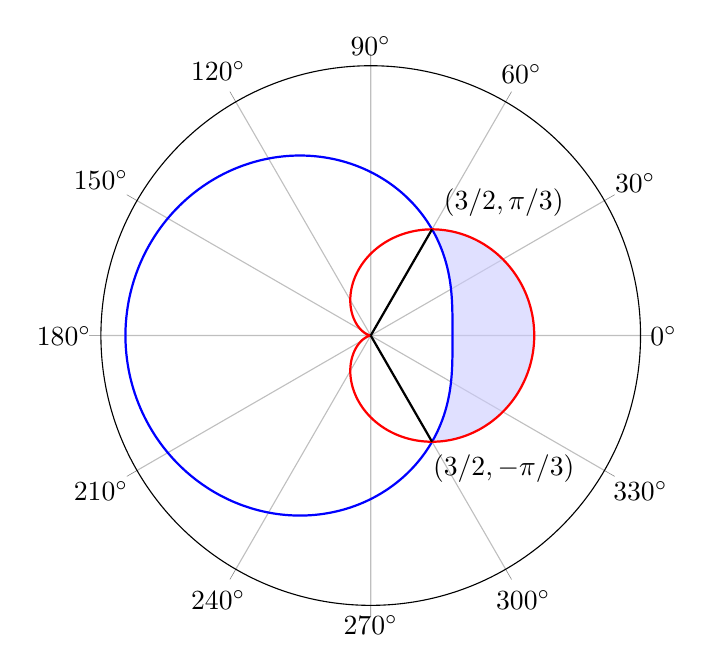
\begin{tikzpicture}
  \begin{polaraxis}[ytick=\empty, axis y line=none, xticklabel=$\pgfmathprintnumber{\tick}^\circ$,]
    \addplot [
      domain=-pi/3:pi/3,
      samples=300,
      draw=none,
      name path=A,
      data cs=polarrad,
    ] {2-cos(deg(x))};

    \addplot [
      domain=-pi/3:pi/3,
      samples=300,
      draw=none,
      name path=B,
      data cs=polarrad,
    ] {1+cos(deg(x))};

    \addplot [
      blue!20,
      fill opacity=0.6,
    ] fill between[of=A and B];

    \addplot [
      domain=0:2*pi,
      samples=300,
      thick,
      blue,
      data cs=polarrad,
    ] {2-cos(deg(x))};

    \addplot [
      domain=0:2*pi,
      samples=300,
      thick,
      red,
      data cs=polarrad,
    ] {1+cos(deg(x))};

    \draw[black, thick] (axis cs: 0,0) -- (axis cs:60,3/2);
    \draw[black, thick] (axis cs: 0,0) -- (axis cs:-60,3/2);
    \node at (axis cs: 45,2.3) {$(3/2,\pi/3)$};
    \node at (axis cs: -45,2.3) {$(3/2,-\pi/3)$};
    
  \end{polaraxis}
\end{tikzpicture}
\end{center}
\begin{align*}
\text{Area}&=\int_{-\pi/3}^{\pi/3}\int_{2-\cos\theta}^{1+\cos\theta}\,r\,dr\,d\theta=\frac12\int_{-\pi/3}^{\pi/3}\left[(1+\cos\theta)^2-(2-\cos\theta)^2\right]\,d\theta\\\\&=\frac12\int_{-\pi/3}^{\pi/3}\left[1+2\cos\theta+\cos^2\theta-\left(4-4\cos\theta+\cos^2\theta\right)\right]\,d\theta=\frac12\int_{-\pi/3}^{\pi/3}\left(6\cos\theta-3\right)\,d\theta \\\\&=\frac12\bigg[6\sin\theta-3\theta\bigg]_{-\pi/3}^{\pi/3}=\frac12\left[6\sin\frac\pi3-3\cdot\frac\pi3-\left(6\sin\left(-\frac\pi3\right)+3\cdot\frac{\pi}3 \right)\right]=\boxed{3\sqrt3-\pi}
\end{align*}

\hfill

\noindent 4. The upper bound is $z=4-x^2-y^2$, while the lower bound is $z=0$. If we project the domain onto the $xy$-plane, we see that the upper and lower bounds for $y$ are $\sqrt{2-x^2}$ and $0$, respectively. For $x$, the integration starts from $0$ and ends at $\sqrt2$. The volume of the object can be evaluated using the following integral.

\begin{equation*}\mathrm{I}=\int_0^{\sqrt2}\int_0^{\sqrt{2-x^2}}\left[4-x^2-y^2-0 \right]\,dy\,dx\end{equation*}

\hfill

\noindent This integral seems a little bit hard. We can switch to polar coordinates for ease. Use the transformation below.

\[
\begin{array}{c}
x^2+y^2=r^2\\
dA=dy\,dx =r\,dr\,d\theta
\end{array}\quad\rightarrow\quad
\begin{array}{c}
0\leq z\leq4-r^2\\
0\leq r\leq \sqrt2\\
0\leq\theta\leq \pi/2\\
\end{array}
\]

\begin{align*}\mathrm{I}&=\int_{0}^{\pi/2}\int_{0}^{\sqrt{2}}\left(4-r^2\right)\,r\,dr\,d\theta=\int_{0}^{\pi/2}\int_{0}^{\sqrt{2}}\left(4r-r^3\right)\,dr\,d\theta=\int_{0}^{\pi/2}\left[2r^2-\frac{r^4}4\right]_{r=0}^{r=\sqrt2}\,d\theta\\\\&=\int_0^{\pi/2}3\,d\theta=\boxed{\frac{3\pi}2}
\end{align*}

\hfill

\noindent 5.

\hfill

\noindent (i)
\begin{center}
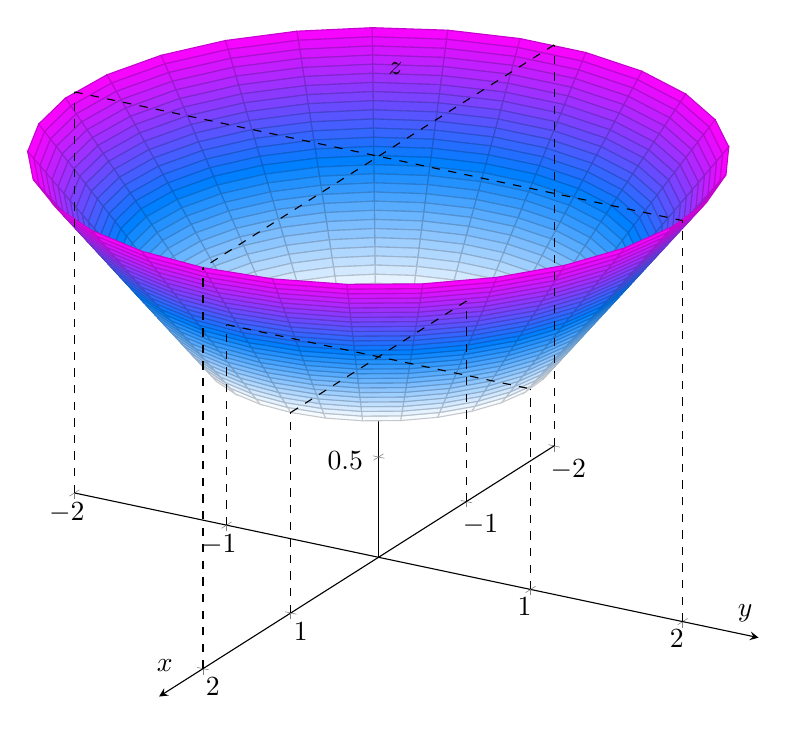
\begin{tikzpicture}
  \begin{axis}[
    view={120}{30},
    axis lines=center,
    xlabel={$x$},
    ylabel={$y$},
    zlabel={$z$},
    xtick={-2,-1,1,2},
    ytick={-2,-1,1,2},
    xmin=-2, xmax=2.5,
    ymin=-2, ymax=2.5,
    zmin=0, zmax=2.5,
    samples=30,
    domain=0:360,
    colormap/cool,
    scale=2,
  ]
    \addplot3[
      surf,
      z buffer=sort,
      y domain=1:2,
    ]
    ({y*cos(x)}, {y*sin(x)}, {y});
%\addplot3[y domain=0:1, dashed, samples = 10]({y*cos(x)}, {y*sin(x)}, {y});
    
\draw[dashed] (axis cs:0,-2,2) -- (axis cs: 0, 2, 2);
\draw[dashed] (axis cs:-2,0,2) -- (axis cs: 2, 0,2);
\draw[dashed] (axis cs:-1,0,1) -- (axis cs: 1, 0, 1);
\draw[dashed] (axis cs:0,-1,1) -- (axis cs: 0, 1,1);

\draw[dashed] (axis cs:-2,0,0) -- (axis cs: -2, 0, 2);
\draw[dashed] (axis cs:0,2,0) -- (axis cs: 0,2,2);
\draw[dashed] (axis cs:2,0,0) -- (axis cs: 2, 0, 2);
\draw[dashed] (axis cs:0,-2,0) -- (axis cs: 0, -2,2);

\draw[dashed] (axis cs:-1,0,0) -- (axis cs: -1, 0, 1);
\draw[dashed] (axis cs:0,1,0) -- (axis cs: 0,1,1);
\draw[dashed] (axis cs:1,0,0) -- (axis cs: 1, 0, 1);
\draw[dashed] (axis cs:0,-1,0) -- (axis cs: 0, -1,1);

\end{axis}
\end{tikzpicture}
\end{center}

\hfill

\noindent (ii) Using the double integral below, we find the lateral surface area.

\begin{align*}
A&=\iint_D\sqrt{1+\left(\frac{\partial z}{\partial x}\right)^2 +\left(\frac{\partial z}{\partial y}\right)^2}\,dA= \iint_D\sqrt{1+\left(\frac{x}{\sqrt{x^2+y^2}}\right)^2 +\left(\frac{y}{\sqrt{x^2+y^2}}\right)^2}\,dA \\\\&=\iint_D\sqrt{1+\left(\frac{x^2+y^2}{x^2+y^2}\right)}\,dA=\iint_D\sqrt{1+1}\,dA=\sqrt{2}\iint_D\,dA
\end{align*}

\hfill

\noindent If we switch to polar coordinates, we can easily evaluate the integral.

\begin{equation*}A=\sqrt2\int_0^{2\pi}\int_1^2\,r\,dr\,d\theta=\sqrt2\int_0^{2\pi}\left[\frac{r^2}2\right]_{r=1}^{r=2}\,d\theta=\sqrt2\int_0^{2\pi}\frac32\,d\theta=\boxed{3\pi\sqrt2}\end{equation*}

\newpage

\noindent 6.

\hfill

\noindent (i) For spherical coordinates, we have

\[
\begin{array}{c}
z=\rho\cos\phi\\
r=\rho\sin\phi\\
x^2+y^2+z^2=\rho^2\\
dV=\rho^2\sin\phi\,d\rho\,d\phi\,d\theta
\end{array}\quad\rightarrow\quad
\begin{array}{c}
x^2+y^2=1\,\rightarrow\,\rho^2\sin^2\phi = 1\\
z=4\,\rightarrow\,\rho\cos\phi=4\\
z=\sqrt{1-x^2-y^2}\,\rightarrow\,\rho\cos\phi=\sqrt{1-\rho^2\sin^2\phi}
\end{array}
\]

\hfill

\noindent We have the lower bound for $\rho$, which is the solution of $\rho\cos\phi=\sqrt{1-\rho^2\sin^2\phi}$.

\[
\begin{array}{c}
\rho\cos\phi=\sqrt{1-\rho^2\sin^2\phi}\implies\rho^2\cos^2\phi=1-\rho^2\sin^2\phi\implies
\rho^2\left(\cos^2\phi+\sin^2\phi\right)=1\\
\rho^2=1\implies\rho=1
\end{array}
\]

\hfill

\noindent However, we have two distinct upper bounds for $\rho$. We need to find the value of $\phi$ where the surfaces $\rho\cos\phi = 4$ and $\rho^2\sin^2\phi=1$ intersect.

\begin{equation*}
\rho^2\sin^2\phi=1 \,\rightarrow\,\rho\sin\phi = 1
\end{equation*}
\[
\left.
\begin{array}{c}
\rho\cos\phi=4\\
\rho\sin\phi=1
\end{array}
\right\}\quad\cot\phi=\implies\phi=\cot^{-1}(4)
\]

\hfill

\noindent For $\displaystyle\phi<\cot^{-1}(4)$, the upper bound is $\displaystyle \frac4{\cos\phi}$. Meanwhile, for $\displaystyle\phi>\cot^{-1}(4)$, it is $\displaystyle \frac1{\sin\phi}$.

\hfill

\noindent The region in the $xy-$plane is circular, therefore $0\leq\theta\leq2\pi$. As for $\phi$, we have $\displaystyle0\leq\phi\leq\frac{\pi}2$. The volume of the object in spherical coordinates can be expressed as follows.

\begin{equation*}
\boxed{\begin{array}{cc}
V=\displaystyle\int_0^{2\pi}\int_0^{\cot^{-1}(4)}\int_1^{\textstyle\frac4{\cos\phi}}\,\rho^2\sin\phi\,d\rho\,d\phi\,d\theta
+\int_0^{2\pi}\int_{\cot^{-1}(4)}^{\pi/2}\int_1^{\textstyle\frac1{\sin\phi}}\,\rho^2\sin\phi\,d\rho\,d\phi\,d\theta 
\end{array}}
\end{equation*}

\hfill

\noindent In fact, we are looking for the minimum value of the upper bound for $\rho$ between $\displaystyle\frac1{\sin\phi}$ and $\displaystyle\frac4{\cos\phi}$. Hence, we can write the equivalent expression as follows.

\begin{equation*}
\boxed{V=\displaystyle\int_0^{2\pi}\int_0^{\pi/2}\int_1^{\min\left(\textstyle\frac4{\cos\phi},\frac1{\sin\phi}\right)}\,\rho^2\sin\phi\,d\rho\,d\phi\,d\theta}
\end{equation*}

\hfill

\noindent (ii) For cylindrical coordinates, we have

\[
\begin{array}{c}
z=z\\
r^2=x^2+y^2\\
dV=r\,dz\,dr\,d\theta
\end{array}\quad\rightarrow\quad
\begin{array}{c}
x^2+y^2=1\,\rightarrow\,r^2 = 1\,\rightarrow\,r=1\\
z=4\\
z=\sqrt{1-x^2-y^2}\,\rightarrow\,z=\sqrt{1-r^2}
\end{array}
\]

\hfill

\noindent The volume can be expressed as follows.

\begin{align*}
    V&=\int_0^{2\pi}\int_0^1\int_{\sqrt{1-r^2}}^{4}\,r\,dz\,dr\,d\theta=\int_0^{2\pi}\int_0^1\big[z\big]_{z=\sqrt{1-r^2}}^{z=4}\,r\,dr\,d\theta\\\\&=\int_0^{2\pi}\int_0^1\left(4r-r\sqrt{1-r^2}\right)\,dr\,d\theta=\int_0^{2\pi}\left[2r^2 + \frac13\left(1-r^2\right)^{3/2}\right]_{r=0}^{r=1}\,d\theta\\\\&=\big[\theta\big]_0^{2\pi}\cdot\left[\left(2\cdot1^2 +0\right)-\left(\frac13+0\right)\right]=\boxed{\frac{10\pi}3}
\end{align*}

\end{document}